% Things to be done before giving away for print
% - spell check
% - let others proof-read

\documentclass[a4paper,twoside]{report}

%% packages
%%%%%%%%%%%
\usepackage[utf8x]{inputenc}
\usepackage[USenglish]{babel}
\usepackage{amsbsy,amscd,amsfonts,amssymb,amstext,amsmath,amsthm,latexsym}
% Package mathpartir is currently not available in nixpkgs
%\usepackage{mathpartir}
\usepackage{stmaryrd}
\usepackage{dot2texi}
\usepackage{tikz}
\usetikzlibrary{shapes,arrows}
\usepackage{url}
\usepackage[xindy]{glossaries}
\usepackage[nottoc]{tocbibind}
\usepackage{pdfpages}

\usepackage{todonotes}

%% options
%%%%%%%%%%
% Currently no such things seem to be needed.
% \newtheorem{definition}{Definition}
% \newtheorem{example}{Example}
% \newtheorem{lemma}{Lemma}
% \newtheorem{theorem}{Theorem}
% \newtheorem{claim}{Claim}
% \numberwithin{definition}{chapter}
\bibliographystyle{alphaurl}
\makeglossaries

%%% Local Variables:
%%% TeX-master: "../thesis"
%%% End:

%% macros
%%%%%%%%%
\newcommand{\loremipsum}{\todo[inline]{Lorem Ipsum}}

%% misc
%%%%%%%%%
\DeclareMathOperator{\pto}{\rightharpoonup}     % partial function arrow
\DeclareMathOperator{\powerset}{\mathcal{P}}    % powerset
\DeclareMathOperator{\proj}{\upharpoonright}    % projection
\DeclareMathOperator{\fst}{\pi_1}               % A x B → A
\DeclareMathOperator{\snd}{\pi_2}               % A x B → B

% Acronyms
%%%%%%%%%%
\newacronym{sdf}{SDF}{Syntax Definition Formalism}
\newacronym{ast}{AST}{Abstract Syntax Tree}
\newacronym{tptp}{TPTP}{Thousands of Problems for Theorem Provers}


%%% Local Variables:
%%% mode: latex
%%% TeX-master: "../thesis"
%%% End:


\begin{document}

% Title page
%%%%%%%%%%%%
\includepdf{titlepage.pdf}

\newpage
\thispagestyle{empty}
\mbox{}

% Erklärung
%%%%%%%%%%%
\input{include/erklaerung}

% Abstract
%%%%%%%%%%
\begin{abstract}
\documentclass{acm_proc_article-sp}

\usepackage[utf8]{inputenc}

\usepackage{cite}

\begin{document}

\title{A Language for the Specification and Efficient Implementation
  of Type Systems}

\numberofauthors{1}

\author{
\alignauthor
Pascal Wittmann
}

\maketitle

\begin{abstract}
  Type systems are important tools to ensure partial correctness of
  programs, to establish abstractions and to guide the programmer in
  the development process. However, there is currently a lack of
  established tools supporting the development of type systems, as
  there are for lexers and parsers. We introduce a declarative
  specification language for type systems, that allows to type systems
  in a natural deduction style. Two results are generated from those
  specifications. A first-order formula representation to facilitate
  the use of automated theorem provers and an efficient type
  checker. Both results aim to support a faster development cycle for
  type systems.
 \end{abstract}

\section{Motivation}
Type systems ensure partial correctness of programs or in other words,
they try to ensure that programs have meaning in the sense of the
semantics of the programming language. The type systems we investigate
are static type systems and can also be thought of as a static
approximation of the program semantics. Besides ensuring partial
correctness, type systems are means to establish abstractions and to
enforce adherence to these abstractions. All in all this can help to
develop software more efficiently
(cf. \cite{Petersen:2014:ECS:2597008.2597152} and
\cite{Mayer:2012:ESI:2384616.2384666}).

Type systems are useful tools, if they fit to the programming language
and their use. To ensure that they fit to the programming language and
their use it makes sense to adapt and modify existing type system or
create new specialized type systems. Those specializations can lead to
better error messages, more expressive type systems and the detection
of more errors. Currently there are, to our best knowledge, no
established tools that generate usable type checkers from declarative
specification languages. Those generators could make the development
of type checkers faster and less error prone. Those generators would
fit well into the language development workbench besides the long
established lexer and parser generators.

The other advantage of generating a type checker from a declarative
specification language is that the specification is close to the
formal description of the type system and the generation of the type
checker can be verified in the absence of a concrete
specification. Often not only the verification of the implementation
is a concern, but also that the type system satisfies certain
properties. As the proofs of propositions about type systems change
when the type system changes, it is desirable to make most of these
changes automatically. Therefore an other motivation for a type
checker generator is to translate specifications into first-order
formulas which can be fed into automated theorem provers to prove
propositions. This establishes a direct connection between the
propositions and the generated type checker.

%% TODO: Mention the application to other kind of type systems?

\section{Research Problem}
The research problem we are trying to tackle is to create a tool that
allows to create an efficient type checker from a declarative
specification and that reduces the gap between formal reasoning about
type systems and their implementation. This problem splits up in
several smaller problems.

The first problem is the design of a declarative specification
language that is close to the formalisms used for type systems. This
language should make it easy to use existing syntax definition of
realistic programming languages and the difference between typing
rules on paper and in the specification language should be small.

The next problem is to investigate a good first-order formula
representation of specification. This representation should be
designed such that it suits automated theorem proving and thus fast
proves. It should also be investigated to which extend theorem provers
for first order logic can be used for type checking.

The main problem is the generation of an efficient type checker. The
performance of the resulting type checker should be comparable with
type checkers that are implemented by hand. The generator should also
be able to cope with non-syntax directed typing rules in an efficient
manner. As one way to achieve this it should be investigated whether
facts proven by an automated theorem prover can be exploited.
\section{Related Work}
\section{Results}
\section{Contributions}

\end{document}
\end{abstract}

% Table of contents
%%%%%%%%%%%%%%%%%%%
\tableofcontents

\todo[inline]{Where do I put the "I would like to thank …"}
\todo[inline]{Search for a better word for 'goal'}
\todo[inline]{How do we refer to all the different types of
  languages? This should be done uniformly.}
\todo[inline]{Use glossary for abbreviations.}

% Content
%%%%%%%%%

\chapter{Introduction}
\section{Motiviation}
\todo[inline]{Somehow mention that we are always talking about static
  type systems}
\todo[inline]{Mention studies on type systems, e.g. by Hanenberg}

Type systems try to solve the problem of ensuring that programs have
meaning. They assign types to expressions and have rules that state
which expressions of which types can be combined. A type checker
ensures that the expressions of a program meet those rules, if those
rules are met, the program is called well-typed. Essentially a type
system ensures that a program has meaning, by approximating its
semantics. They also can be used to establish abstractions and to
enforce the adherence to these abstractions.

Although type systems are a useful tool increase software quality,
there is a lack of tools that help to create and modify type
checkers. Almost all type checkers are implemented by hand and are far
away from their formal models. In addition it is non-trivial to write
or even extend a type checker. Therefore current tools are not suited
for quick prototyping of type system features for new or existing
languages. This is also true for the development of domain specific
languages (DSL). In that sense type systems are underprivileged in
comparison to parsers. Parser generators are widely spread and
accepted tools.

The goal of this thesis is to close that gap in the tool chain. A
declarative specification language is developed, in which type systems
can be represented very close to the standard formalisms. Two things
are generated from those specifications. First, a representation of
the type system as first-order formulas, intended to support proving
properties of the type system. Second, an efficient type checker that
can be integrated in existing tool chains.
\section{Contributions}
The main contributions of this thesis are:
\begin{enumerate}
\item A declarative specification language for static type systems, in
  which typing rules can be written in the style of natural deduction
  and which builds SDF definitions of programming languages.
\item The transformation of type system specifications into equivalent
  first-order formulas in the TPTP format, suitable to be passed to
  automated theorem provers.
\item A generator that creates type checkers from type system
  specifications and which is designed for performance.
\end{enumerate}

\section{Structure}
\todo[inline]{Describe how the thesis is structured.}

%%% Local Variables:
%%% mode: latex
%%% TeX-master: "../thesis"
%%% End:
\chapter{Preliminaries}
\section{Tools}
This section introduces the tools used in this thesis. We argue what
makes the tools suitable for achieving the goals of the thesis and
give a short overview of the alternatives.

\subsection{SDF}
\gls{sdf}~\cite{Heering:1989:SDF:71605.71607} is a formalism to define
the syntax of formal languages in the tradition of
\gls{bnf}. \gls{sdf} allows to define lexical and context-free
grammars and is, in contrast to \gls{bnf}, modular. This modularity
allows to compose \gls{sdf} syntax definitions. There are also parser
generators for \gls{sdf}, see~\cite{Rekers92parsergeneration}. In
contrast to formalisms for traditional parser generators like
Yacc~\cite{Johnson75yacc:yet}, \gls{sdf} specifications are purely
declarative, which increases the reusability of the specifications.

The modularity of \gls{sdf} is a consequence of the fact that
\gls{sdf} is \textit{generalized LR
  parsable}~\cite{Rekers92parsergeneration}. Generalized parsing means
that parsing might be indeterminate, i.e.\ the parser produces all
possibilities for syntactic ambiguities. This might not seem to be an
advantage, but generalized parsing has some nice implications. First,
the class of supported grammars is bigger and therefore enforces less
restrictions on the programmer and might allow a natural definition of
languages. Second, it enables the modularity of \gls{sdf}, because the
composition of generalized LR grammars is a generalized LR
grammar. This does not hold in general for LR grammars.

An other advantage is that \gls{sdf} is also scannerless
parsable~\cite{Brand02disambiguationfilters}, that means that
tokenization and parsing can be done in a single step.

\gls{sdf} also has support to specify layout sensitive
languages~\cite{conf/sle/ErdwegRKO12} like Python or Haskell. It
enforces context insensitive layout constraints at parse time and
context sensitive constraints at disambiguation time, i.e.\ all
ambiguities that violate layout constraints are removed.

\begin{figure}
\begin{example}{~}
\begin{lstlisting}[language=sdf]
module Bool
exports
  context-free start-symbols Bool
  sorts Bool
  context-free syntax
    "true"  -> Bool
    "false" -> Bool
    "~" Bool -> Bool {cons("Not")}
    Bool "&" Bool -> Bool {cons("And"),
                           layout("2.first.col < 2.left.col")}
\end{lstlisting}
\label{ex:sdf-grammar}
\end{example}
\end{figure}

Example~\ref{ex:sdf-grammar} shows a grammar that allows to write
conjunctions of \code|true| and \code|false|. Conjunctions are
represented in the \gls{ast} with the constructor \code|And| and the
layout constraint enforces, that if conjunctions span over multiple
lines, the right-hand side of \code|&| needs to be indented.

\gls{sdf} is used in this thesis to define the syntax of the
specification language for type systems and for the target
languages. Features like layout constraints make \gls{sdf} a good tool
for defining complex syntax for natural deduction rules. The
modularity and composability make it possible to define the syntax of
the specification language independent of the target language.

\subsection{Stratego/XT}
Stratego~\cite{Visser01} is a framework for the development of
transformation systems. It consists of the transformation language
Stratego and a set of tools (XT) for tasks like parsing and pretty
printing. The paradigm of Stratego is to use user-definable strategies
for rewriting. Stratego distinguishes the following abstraction
levels.

\begin{description}
\item[Transformation rules] are basic rewrite rules on the structure
  of the \gls{ast}.
\item[Transformation strategies] are the glue between the
  transformation rules. They combine rules, define the order of
  application and the traversal order of the \gls{ast}. These
  strategies can be defined generically. \textit{scoped dynamic
    rewrite rules}~\cite{Visser01scopeddynamic} pass context
  information during the traversal, because normal rewrite rules are
  context-free.
\item[Transformation tools] allow to compile transformation strategies
  into a stand-alone program. The interface between such programs is
  the ATerm format for \glspl{ast}.
\item[Transformation systems] describe a set of programs created by
  the transformation tools. A transformation system for a
  source-to-source transformation usually includes a parser and pretty
  printer.
\end{description}

Example~\ref{ex:stratego-module} shows a Stratego module that declares
the constructors from Example~\ref{ex:sdf-grammar}. It has one rule
\code|Eval| that reduces a term one step. The strategy \code|eval|
applies rule \code|Eval| repeatedly from bottom to top.

\begin{figure}
\begin{example}{~}
\begin{lstlisting}[language=stratego]
module Bool
signature
  sorts Bool
  constructors
    Not   : Bool -> Bool 
    And   : Bool * Bool -> Bool
rules
  Eval : Not(True)      -> False
  Eval : Not(False)     -> True
  Eval : And(True, x)   -> x
  Eval : And(x, True)   -> x
  Eval : And(False, x)  -> False
  Eval : And(x, False)  -> False
strategies
  eval = bottomup(repeat(Eval))
\end{lstlisting}
\label{ex:stratego-module}
\end{example}
\end{figure}

Stratego interacts well with \gls{sdf} and has facilities to integrate
into tool-chains. In addition it allows to write abstract and generic
transformations. That makes it a good choice for the transformation
system.

\subsection{Spoofax}
Spoofax~\cite{KatsV10} started with the goal to provide an \gls{ide}
for \gls{sdf} and Stratego. It was then developed to a language
workbench for Eclipse that allows language development with editor
support for both, the languages used for development and the developed
language. Spoofax allows smooth switching between both editor
services. The editor for the developed language can be deployed
standalone. Those editor services can provide syntactic and semantic
analysis based on live parses, with error recovery and origin
tracking. Those facilities are implemented language pragmatic, which
allows developers to focus on language specific parts.

We use Spoofax in this thesis to provide editor support for the
specification language and as glue between \gls{sdf} and Stratego in
the development of the specification language, the formula generator
and the type checker generator.

\subsection{Vampire}
We use the automatic theorem prover Vampire~\cite{VoronkovVampire} to
proof classical first-order logic propositions about type system
specifications. Vampire is able to parse formulas in the \gls{tptp}
format and provides detailed output for the conducted proofs. We use
this output to extract information about the applied axioms, which are
in our case typing rules.

\subsection{Alternatives}
We chose Spoofax and its components, because its feature set fit well
to our goals and there was some previous work related work based on
it. However there are alternative \textit{language workbenches} that
could have been a good fit as well. For example
Rascal~\cite{klint2009rascal} a meta-programming language that has
among others support for context-free grammars, algebraic data-types,
relations, relational calculus operators, advanced patterns matching,
generic type-safe traversal, comprehensions, and string templates for
code generation.~\cite{workbenches} gives an overview of the state of
the art in language workbenches.

\section{Type Systems}
\textit{Type theory} started as an attempt by Gottlob Frege to solve
Russel's paradox, that shows that \naive{} set theory is
inconsistent. Frege argued that a predicate requires an object as
argument and cannot have itself as an argument, as it is the
subject. So the initial motivation for type theory was to avoid
paradoxes and contradictions in logics and rewrite systems. The term
\textit{type system} refers to type theories whose logics rewrite
systems are programming languages. Type systems address the problem to
ensure that programs have meaning, whereas in type theory the problem
is the ensure the consistency of a logic.

What does it mean to ``ensure that programs have meaning''. First, it
means that one wants to filter the useful programs. It is not useful
to have a syntactically valid program that has no semantics. A type
system assigns types to the expressions of the programming language. A
\textit{type checker} can then check, whether the types of the
programs expressions match according to predefined typing rules. If
the type checker succeeds the program is \textit{well-typed} and has
meaning, i.e.\ the program will not exit due to undefined
semantics. Depending on the expressiveness of the type system also the
correctness of the computation that the program performs can be shown.

\section{First-Order Logic}

%%% Local Variables: 
%%% mode: latex
%%% TeX-master: "../report"
%%% End: 


\chapter{Specification Language}
The goal of this thesis is to create a generator for type checkers,
like there are generators for lexers and parers. Such a generator can
only be a useful tool, if the specifications from which the type
checkers are generated are easy to read and write for people who are
familiar with type systems and if the specification language is
expressible enough to handle real-world languages. As there is no
common format for type system specifications, a new specification
language was designed with the following goals in mind:

\begin{enumerate}
\item Close to the formal or mathematical notations that are commonly
  used to close the gap between the formal model and the
  implementation side.
\item Declarative, makes it easy to try things out and increases
  maintainability and readability of specifications.
\item Modularity, it should be possible to combine type systems to
  increase reuse.
\item Existing programming language definitions should integrate nicely.
\end{enumerate}
\section{Design \& Architecture}
A specification is divided into eight sections, of which two are
optional. The three sections are for organizational purposes. The
first section declare the name of the specification. This name is a
unique identifier and used for imports. The second section declares
which other specifications are imported. The third section declares
the language for which a type system should be specified. This
language needs to be present in SDF and there must be a module with
exactly that name. \todo[inline]{Does it make sense to allow imported
  files to declare a language?}

In the fourth section meta-variables are declared. The declaration of
a meta-variable consists of an identifier, of a prefix and of a set of
non-terminals of the base language. The identifier can be used to
distinguish different kinds of meta-variables.\todo{Currently this is
  not used} A meta-variable can consist of letters and numbers, to
ensure that we can parse meta-variables of different kinds
unambiguously every meta-variable must be prepended with the declared
prefix. As we want to introduce meta-variables at different positions
in the base language we need a way to extend the syntax of the base
language. The set of non-terminals in a meta-variable definition lists
the non-terminals that shall be extended.

\todo[inline]{Make up my mind about the name of those environments}
In the fifth section all environments that will be used in the
judgments are defined. Informally these environments are declared as
cross-products of non-terminals, i.e. an environment is a set
consisting of pairs of terminals that can be produced by the
non-terminals in the declaration. Every environment has a name, which
can be used in further declarations. Lookups may differ for
environments and use cases, therefore one has to annotate the
non-terminals with input and output tags. Terminals at positions that
are tagged with input are used to look up terminals tagged with output
that are saved in the environment. An environment for which all
non-terminals are tagged with input, is equivalent to a normal look up
in a set and will return whether the tuple could be found. An
environment with only outputs acts as a sink, one can put things into
it, but never retrieve anything back.

The sixth section declares type judgments. Type judgments can be
declared in a flexible way, non-terminals can be mixed arbitrarily
with separators. This allows the programmer\todo{Is this the right
  word?} to declare the type judgments as close to formalizations as
possible. As for environments the non-terminals in the type judgments
have to be annotated with input/output-tags to determine what should
be computed.

In the last two sections the typing rules and conjectures are
declared. Both typing rules and conjectures have the same
syntax. Typing rules specify the type system and conjectures are used
to provide test cases and are optional. A typing rule consists of a possible empty list
of typing judgments, an optional name and a typing judgment as
conclusion.

\begin{figure}
\begin{verbatim}
module example
imports common
language simply-typed-lambda-calculus
meta-variables 	Term "~" { Type Exp }
                Ctx "$" { Context }
                Id "%" { ID }
contexts Context := ID{I} x Type{O}
judgments Context{I} "|-" Exp{I} ":" Type{O}.
rules

%x : ~T in $C
============== T-Var
$C |- ~x : ~T

(%x : ~T ; $C) |- ~t : ~T
================================= T-Abs
$C |- \ %x : ~T . ~t : ~T -> ~T

$C |- ~t1 : ~T11 -> ~T12
$C |- ~t2 : ~T2
========================= T-App
$C |- ~t1 ~t2 : ~S
\end{verbatim}
\caption{Specification for a type system for the simply typed lambda calculus}
\end{figure}
\section{Implementation}

%%% Local Variables: 
%%% mode: latex
%%% TeX-master: "../report"
%%% End: 

\chapter{Formula Generation}
\label{ch:formula-generation}
Type systems in programming languages can be treated as black boxes
from a programmers point of view. The programmer interacts with the
type system for example via type annotations and receives feedback
from the type system in form of error messages. Errors in the type
system are hard to detect for the programmer, because he cannot be
sure if it is an error in his program or in the type system (or its
implementation). In addition he can only debug his program, because of
the black box view on the type system. Therefore it is desirable to
ensure that the type system has the intended semantics.

Mathematical proofs are used to ensure that a type system has the
intended semantics. A basic property of type systems is safety, which
roughly says ``a well-typed term can never reach a stuck state during
evaluation''\todo{Cite Pierce}. Those properties can be proven by
hand or with the help of proof assistants. Both methods require
substantial manual effort. In accordance to the goal of the automated
generation of type checkers, we explore how well automated theorem
provers can solve simple propositions and how this can be exploited in
the type checker generation. We generate formulas from type system
specifications to interface with automated theorem provers.
 
\section{Goals}
With generation formulas from type system specification we pursue two
goals. The first goal is to resemble type system specifications
in formulas suitable for automated theorem provers and to use this as
a basis to prove simple properties. The second goal is to explore how
well automated theorem provers can check if a program is well-typed.

\section{Why First-Order Logic?}
\subsection{Expressiveness}
\subsection{Tool-Support}
\section{Translations}
\label{sec:translations}
For the generation of first-order formulas not all sections of a
specification are important. The section that declares the
meta-variables and the section that declares the judgments are not
used at all. With regard to formula generation they are only used to
ensure correct syntax.

The following parts of a type system specification are translated into
first-order formulas as described below: Environments, AST nodes of
the programming language, meta-variables and typing rules.

\todo[inline]{Implement imports and describe how they are handled.}

Environments declarations are translated in a uniform way. For every
environment two formulas are generated. These two formulas model the
look-up of entries in the environment, which is equivalent to how they
are stored. Those formulas have an inductive nature, one formula
models the base case and the other one the step case for the lookup.

%% FIXME: This seems to be no good way to refer to formulas. How is it
%% done right? Haven't found an example in my bachelor thesis by chance.
\begin{figure}
\label{formula:environment-base}
\begin{multline}
  \forall e, x_1, \dots, x_n, y_1, \dots, y_m . \\
  (lookup_e(x_1,\dots,x_n,y_1,\dots,y_m,
  bind(x_1,\dots,x_n,y_1,\dots,y_m,e)))
\end{multline}
\end{figure}

The formula \ref{formula:environment-base} represents the base case of
environment look-ups. All non-terminals in the environment definition
tagged as input are translated into variables $x_1 \dots x_n$ and all
tagged as output are translated into variables $y_1 \dots y_m$,
respectively. The variable $e$ ranges over all possible
environments. The $bind$ predicate used in this formula models the
binding of new input/output pairs to the environment. In the
implementation the order of arguments is a bit different, but this
difference is for the discussion of the concept negligible. For
details see Section \ref{sec:implementation-fof}. The predicate
$lookup$ models the lookup in the environment. It is used to check
whether some input/output pair exists in the environment. In the base
case the an input/output pair is added to an environment $e$ and
looked-up directly afterwards. Therefore the look-up succeeds as the
required elements are directly given in the bind predicate.

\todo[inline]{Format look-up step formula nicely.}
\begin{figure}
\label{formula:environment-step}
\begin{multline}
  \forall e, x_1, \dots, x_n, x_1', \dots, x_n', y_1, \dots, y_m,
  y_1', \dots,
  y_m' . \\
  (x_1 \neq y_1) \land \dots \land (x_n \neq y_n) \land (lookup(x_1,
  \dots, x_n, y_1, \dots, y_m, e) \implies \\ lookup(x_1, \dots, x_n,
  y_1, \dots, y_m, bind(x_1',\dots,x_n',y_1',\dots,y_m',e))
\end{multline}
\end{figure}

Formula \ref{formula:environment-step} models the step case of
environment look-ups. The intuition is that if some input/output pair
is contained in an environment $e$ the it is also contained in an
environment in which in addition a different input/output pair is
stored. Variables $x_i$ and $x_i'$ are non-terminals from the
environment declaration tagged with input, $y_i$ and $y_i'$ are
non-terminals tagged with output respectively.

The AST nodes of the programming language are translated directly into
predicates. For the translation the following scheme is used. Assume
an AST node of the following form $Cons(e_1, \dots, e_n)$ is
translated into a predicate of the form $cons(p_1, \dots, p_n)$, where
all consituents $e_i$ are translated into predicates $p_i$
recursively. To help theorem provers for each of those predicates an
axiom for injectivity and univalence is created. Those hold by
definition of the AST nodes.

The most important part is the translation of the typing
rules. Depending on whether the typing rules has premises either of
the following schema is used:

\begin{figure}
\label{formula:typing-rule}
\begin{align}
  &\forall FV(c) .& c \\
  &\forall FV(p_1,\dots, p_n, c) .& p_1 \land \dots \land p_n \implies c
\end{align}
\end{figure}

\todo[inline]{In the following free variables are actually free
  meta-variables.}
The meta-variables $p_i$ are the premises and $c$ is the conclusion of
the typing rules. The intuition of a typing rule is that the
conclusion can be derived if all premises can be derived. In terms of
first-order logic ``derived'' means for arbitrary formulas that there
is a proof and for predicates that the predicate holds under the given
interpretation. Therefore a typing rule without premises is translated
into a formula that consists of the conclusion and all-quantifies all
free variables of the conclusion. Free variables are all-quantified,
because all possible variants of the conclusion have to be derivable.
Typing rules with premises are translated into a single
implication. The premise of the implication is the conjunction of all
premises of the typing rule. This ensures that all premises need to be
derivable/satisfied. The conclusion of the implication is the
conclusion of the typing rule. This makes sense as the intuition was,
that the conclusion of the typing rule is derivable if all premises
are derivable, which is exactly the semantics of this implication.

Type judgments are translated into simple predicates. Equality and
inequality can be expressed via judgments with the annotation ``is
Eq'' and ``is Neq'', respectively. Those judgments must have exactly
two non-terminals.
\section{Implementation}
\label{sec:implementation-fof}
The implementation details of the translation from the specification
language into first-order formula is described in this section.

\todo[inline]{Extend for imports.}
The implementation is organized in the following steps. Fist, the
module is split up into its components. Those are: module description,
imports, programming language, meta-variables, environments,
judgments, typing rules and conjectures. Second, environments, typing
rules and conjectures are transformed into first-order
formulas. Third, for each conjecture a file is created which contains
all generated formulas. In the following those steps are explained in
detail.

The module is split up by pattern matching. For formula generation
only the environment definitions, typing rules and conjectures are
used.

Formulas for the environment definitions are generated for each
environment definition separately and are added to the axioms. The
non-terminals of an environment definition are indexed with fresh
names. Those fresh names will be used as variables in the first-order
formulas. The structure of the formulas, as it is defined in
\ref{formula:environment-base} and \ref{formula-environment-step}, is
hard-coded in the internal representation for first-order formulas. To
adhere to this structure the variables representing the non-terminals
are split up by their input/output attribute. The counter parts for
the variables needed in the step case are created by appending an
underscore to the variable name, as a tick is not valid in TPTP.

Rewriting typing rules into first-order formulas is the most complex
process in the formula generation. The rewrite process is triggered
when a typing rule is encountered. When a typing rule with premises is
encountered the premises and conjectures are rewritten by the strategy
\texttt{rewrite}. Premises are, due to limitations of the
\texttt{layout}-rules, not represented as ordinary lists after
parsing. Therefore these special lists are transformed into an
ordinary list by the generic \texttt{to-list} strategy. Then the
free variables of premises and constraints are collected. Now an
implication is constructed from the list of premises and the
conclusion and in the case there are free variables, those variables
are all quantified. By now the constructed formula has the structure
shown in \ref{formula:typing-rule}.

Now the details of the \texttt{rewrite} strategy are presented. This
strategy is defined as a sequence of two top down traversals. The first
traversal is the actual rewrite of the typing judgments and the second
is a special treatment for strings. The first traversal is organized
as follows. An attempt to rewrite the current node into an auxiliary
constructor is made, if this attempt succeeds the auxiliary
constructor is rewritten into a term of the first-order formula
language, if it does not succeed it is wrapped into the \texttt{Term}
constructor. The reasoning is the following. Some AST nodes of the
specification language are generic, those referring to the environment
formulas, to the typing judgments and to the meta-variables. Those
consist of some constant string plus some user defined
string. Therefore it is not possible to use normal pattern matching on
them. The only chance to cope with them is to use the generic
\texttt{cons\#(args)} pattern, to access the name of the constructor
as a string. The auxiliary constructor \texttt{AuxCons} is used to
abstract over this generic pattern. The rule \texttt{makeAuxCons}
splits the constructor name into the constant string and the user
defined one and provides the arguments as they are. After this
transformation it is possible to use normal pattern matching on
\texttt{AuxCons}. \texttt{makeAuxCons} only succeeds on the
constructors mentioned before. If a node can be transformed into an
auxiliary constructor the constructor is rewritten immediately
afterwards into a constructor of the first-order logic target
language. These rewritings are trivial mappings from auxiliary
constructors to constructors of the target language. If a
transformation into an auxiliary constructor is not possible, the
current node is wrapped into a \texttt{Term} constructor if it is not
a constructor of the target language. The constructor \texttt{Term}
indicates that the wrapped constructor is a constructor of the
programming language, i.e. no constructor of the specification, nor of
the target language. This wrapping is needed for controlled pretty
printing of programming language constructors. In the second top down
traversal strings in the arguments of predicates (\texttt{Pred}) and
term (\texttt{Term}) constructors are wrapped into a \texttt{Term}
constructor to handle constructors without parameters. This wrapping
is needed later on to provide inequalities of constants symbols.

The rewriting of typing rules and conjectures is very similar,
therefore only the differences to the rewriting of typing rules are
described. Conjectures are as their name suggests rewritten into
formulas tagged as conjectures and are therefore also named
\texttt{goal} if no name is specified. \todo[inline]{Are there more
  differences}

\section{Performance}
%%% Local Variables: 
%%% mode: latex
%%% TeX-master: "../report"
%%% End: 

\chapter{Type Checker Generation}
\section{Goals}
In this section we briefly describe and motivate the design and goals
of the type checker generator.

The first goal is to generate type checkers from high level type
system specifications that are not geared to type checking. Mainly
this means to try to deal with non-syntax directed typing rules
without backtracking. The motivation for this is that non-syntax
directed typing rules are often more readable and that changes have
mainly local effects. 

The second goal is to design a modular type checker generator,
particularly one that can be easily adapted and that facilitates the
exchange of components. This modularity is desirable because it
increases the reusability and makes it possible to combine previously
unrelated projects.

The third goal is to generate type checkers that emit readable error
messages if a program is not well-typed. This is essential to make the
generated type checker usable in production in any way.
\section{Architecture}
The type checker generator has two phases: Template generation and
template optimization. The template generation phase transforms the
type system specification with modifications into templates. A
template is a different representation for a typing rule that is
better suited for type checking. We introduce templates in detail in
Section~\ref{sec:constraint-templates}. The template optimization
phase checks which optimizations apply to the generated templates and
applies them. The optimizations aim to reduce the amount of
non-determinism in the type system and therefore reduce the amount of
backtracking in the type checker. The final product after those two
phases is a file that contains the optimized templates.

The template optimization phase is the key part of the type checker
generator. It is the link between the type checker generator on the
one hand and the formula generation and automated theorem provers on
the other hand. We generate from a single type system specification a
first-order formula representation suitable for theorem proving and a
template representation suitable for constraint generation. In the
optimization phase we combine them by using the automated theorem
prover to check if optimizations are applicable to the templates.

Instead of generating a type checker directly from the specification,
we implement a generic constraint-based type checker that takes
templates as input. This generic type checker has two phases:
Constraint generation and constraint solving. The constraint
generation phase takes the templates and the expression that shall be
type checked as input. We then build a derivation tree according to
the expression by pattern matching the conclusion of the
templates. The building and traversing of the derivation tree emits
constraints. In the constraint solving phase we then try to unify the
emitted constraints. If that succeeds it reports the result otherwise
it reports the errors that occurred during unification.

Figure~\ref{fig:phases} shows the phases and their
relationships. Nodes represent phases and arrows express that data
flows from one node to another. Labels on arrows describe the data
format.

The four phases correspond to modules or tools. Each phase has a
well-defined interface, therefore the implementation can be exchanged
freely. This facilitates the use of different constraint solvers,
constraint generators or template optimizers.

\begin{figure}
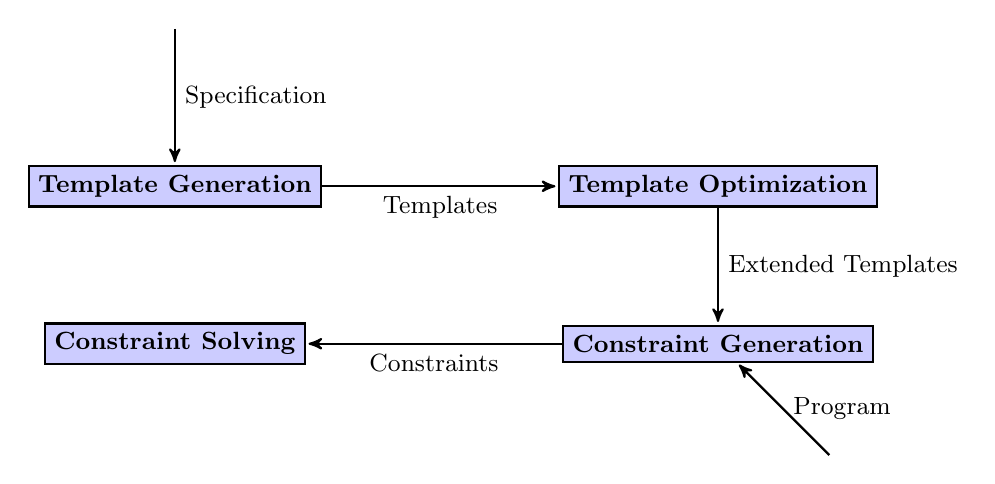
\begin{tikzpicture}[->,>=stealth',shorten >=1pt,auto,align=center,node distance=2cm,
  thick,main node/.style={rectangle,fill=blue!20,draw,font=\small\bfseries}]

  \node[main node] (1) {Template Generation};
  \node[main node] (2) [right=3cm of 1] {Template Optimization};
  \node[main node] (3) [below of=2] {Constraint Generation};
  \node[main node] (4) [below of=1] {Constraint Solving};
  \coordinate [below right of=3] (5);
  \coordinate [above of=1] (6);

  \path[every node/.style={font=\small}]
    (1) edge node [right, below] {Templates} (2)
    (2) edge node [right] {Extended Templates} (3)
    (5) edge node [right] {Program} (3)
    (3) edge node [right, below] {Constraints} (4)
    (6) edge node [right] {Specification} (1);
\end{tikzpicture}
\caption{Phases of the type checker generator}
\label{fig:phases}
\end{figure}

The following sections describe the implementation of the type checker
generator. Each section focuses on one of the phases.

\section{Template Generation}
\label{sec:constraint-templates}
The first phase translates type system specifications into
templates. This phase is not just a simple translation from a human
readable representation into a representation suitable for programs,
but also normalizes the resulting templates. Normalization comprises
the elimination of implicit equalities and resolves dependencies
between premises. All following phases assume normalized templates.
The normalization allows simplifications in the implementations of the
phases.

\subsection{Templates}
A template is an intermediate representation of a typing rule that is
more suitable for the constraint generation process and defined in
Definition~\ref{def:template}.

Templates serve as the input format for the constraint generation
phase of the type checker. Besides being better suited for constraint
generation templates also have the advantage that we can adapt the
system to other specification languages by translation into
templates. The structure of the templates has no hard requirements on
the specification language, although it has to be declarative. In
general the structure of the templates is similar to the structure of
the typing rules of the specification language.

\begin{figure}
\begin{definition}{Definition of the syntax of templates}
  The Stratego implementation appends to all constructors two
  underscores to avoid name collisions with target languages. This is
  necessary as the module system of Stratego is not strong enough to
  avoid those collisions. We omit these here for the sake of
  readability. The non-terminals Inputs, Outputs, Term and Error may
  contain arbitrary terms.
  \begin{grammar}
    <Template> ::= `Template' <Premises> <Conjecture>

    <Conjecture> ::= `Conjecture' <Judg> <Name> <Pattern> <Outputs>

    <Premises> ::= $\epsilon$ | <Premise> <Dependencies> <Premises>

    <Premise> ::= `Lookup' <Ctx> <Inputs> <Outputs> <Error>
    \alt `Judgment' <Judg> <Inputs> <Binding> <Outputs> <Error>
    \alt `Eq' <Term> <Term> <Error>
    \alt `Neq' <Term> <Term> <Error>

    <Dependencies> ::= $\epsilon$ | <Judg> <Outputs> <Dependencies>

    <Name> ::= `Some' <String> | `None'

    <Judg> ::= <Int>
  \end{grammar}
\label{def:template}
\end{definition}
\end{figure}


Before we are going to describe the structure of templates in depth,
we highlight the conceptual differences between templates and typing
rules. Templates take advantage of the input/output tags of typing
judgments and context definitions by splitting everything up into an
input and output part. This will become handy in the constraint
generation phase, where we can see immediately which are the patterns
to match against the expressions and which are the output positions
that we have to compute. As described in the introduction to this
chapter, we also normalize templates. For each implicit equality in
the conclusion and premises of typing rules we add an explicit
equality. Thus every variable occurs in each judgment only
once. Further we sort premises by dependencies between their
inputs/outputs. We describe and motivate the normalization process in
the remainder of the section. The template optimization and constraint
generation phase take advantage of these normalizations and therefore
expect their inputs to be normalized.

Note: We transform all meta-variables of the specification into the
variables (\code|Var(name)|) that we use for constraint generation as
we do not need the additional information of meta-variables anymore.

\subsubsection{Premises in Templates}
Premises in templates have multiple shapes: Judgments, context
lookups, equalities and inequalities. A premise always has a (possibly
empty) list of dependencies. This list contains the number and the
outputs of the judgment the premise depends on. Later on in this
section we define what it means for a premise to have dependencies,
first we take a look at the different kinds of premises.

\begin{description}
\item[Judgments] correspond to the user defined judgments of the
  specification. They consist of the judgment number
  \refcallout{judgment:number} which refers to the position in the
  declaration section of the specification, the positions of the
  judgment marked as inputs \refcallout{judgment:inputs}, context
  modifications \refcallout{judgment:bind},
  \refcallout{judgment:reset}, \refcallout{judgment:identity}, the
  output positions of the judgments \refcallout{judgment:outputs} and
  potentially error messages \refcallout{judgment:errors}.

  The main difference between context modifications in templates and
  typing rules is that all modifications are at one place and can
  always be evaluated in the same manner. A context modification can
  either be an addition to a context \refcallout{judgment:bind} which
  consists of a context identifier (this identifier refers to the
  position in the declaration section of the specification), a list of
  inputs and a list of outputs. It can also be a context identity
  \refcallout{judgment:identity} which corresponds to a context
  meta-variable in the specification and context identities do not
  modify the context and a reset operation \refcallout{judgment:reset}
  which resets the given context and corresponds to the empty
  context. Read to context modifications from right to left to obtain
  a valid context. A detail explanation of the semantics in our type
  checker will follow in Section~\ref{sec:constr-gener}.

\begin{example}{~}
\begin{lstlisting}[language=sltc]
Judgment(
        1 %*\callout{judgment:number}*)
      , [Var("X0")] %*\callout{judgment:inputs}*)
      , [ Binding(1, [Var("X1")], [Var("X2")]) %*\callout{judgment:bind}*)
        , Reset(1) %*\callout{judgment:reset}*)
        , Ctx(2) %*\callout{judgment:identity}*)
        ]
      , [Var("X3")] %*\callout{judgment:outputs}*)
      , Some([Error([Var("X0"), "has type", "{}"])]) %*\callout{judgment:errors}*)
      )
\end{lstlisting}
\label{ex:judgment}
\end{example}

In example~\ref{ex:judgment} we have judgment one that has only one
input position \code|Var("X0")| and one output position
\code|Var("X3")|. It leaves context two as it is, resets context one
and then adds the input/output pair \code|Var("X1")| and
\code|Var("X2")| to context one. In addition it is annotate with one
error message.

\item[Context lookups] consist of the context number
  \refcallout{lookup:ctx}, of the input \refcallout{lookup:inputs} and
  of the output \refcallout{lookup:outputs} positions of the context
  lookup from the specification and potentially of error messages
  \refcallout{lookup:errors}. We do not treat look ups as normal
  judgments as their semantics is not defined within the
  specification. Therefore we have to deal with them separately in the
  type checker.

\begin{example}{~}
\begin{lstlisting}[language=sltc]
Lookup(
        1 %*\callout{lookup:ctx}*)
      , [Var("X0")] %*\callout{lookup:inputs}*)
      , [Var("X1")] %*\callout{lookup:outputs}*)
      , None() %*\callout{lookup:errors}*)
      )
\end{lstlisting}
\label{ex:lookup}
\end{example}

  In example~\ref{ex:lookup} we look up \code|Var("X0")| from
  context one and bind the result to \code|Var("X1)"|. This context
  lookup has no error messages attached.

\item[(In)equalities] are predefined judgments and therefore treated
  separately. They have a judgment number, exactly two input
  positions, no output positions and potentially an error message. The
  judgment number is used to keep track of the non-terminals of the
  (in)equality.

\begin{example}
\begin{lstlisting}[language=sltc]
Neq(4, Var("X0"), Var("X1"), None())
\end{lstlisting}
\label{ex:neq}
\end{example}

In example~\ref{ex:neq} we test if \code|Var("X0")| and
\code|Var("X1")| are not equal and provide no error message.
\end{description}

In some cases it is relevant in which order we evaluate premises. As
we have not talked about evaluation yet, we assume premises are
evaluated like functions. We provide terms for input positions an
retrieve terms for the output positions. If we take a look at
Example~\ref{ex:premise-dependencies} we see that typing rule
\code|T-Tapp| from Appendix~\ref{appendix:systemf} has two
premises. When we compare the premises with the judgment definitions,
we see that \code|%x| occurs as an input of the first
premise and as within an output position of the second premise, but
not at all in the conclusion. If we want to evaluate the first premise
we have to find a term for
\code|%x|, but that term is only provided by
the output of the second premise. Therefore we have to evaluate the
second premise first.

\begin{example}{~}
\begin{lstlisting}[language=sltc]
judgments
TermBinding{I} "|" TypeBinding{I} "|-" Exp{I} ":" Type{O}.
Type{O} "= [" ID{I} "->" Type{I} "]" Type{I}.

rules
~U = [ %x -> ~S ] ~T
$C1 | $C2 |- ~e : all %x . ~T 
============================== T-Tapp
$C1 | $C2 |- ~e [ ~S ] : ~U
\end{lstlisting}
\label{ex:premise-dependencies}
\end{example}

We make those dependencies visible in the template language by
annotating each premise with a list of its dependencies. Those
dependencies contain the number of the premise on which the premise
depends and the output positions of that premise. The outputs are
redundant information and only added to make it easier to check which
information are proivded by that dependency.
The dependency for the first premise in
Example~\ref{ex:premise-dependencies} the would look like
\code|(1,[TAll(Var("X0"), Var("X1"))])|. In this example
\code|TAll(Var("X0"), Var("X1"))| is the only output provided by the
premise and \code|1| refers to the second premise, because we sort
premises of templates topological according to the dependencies, as we
will describe in the next section.

\subsubsection{Conclusions in Templates}
Conclusions contain the judgment identifier
\refcallout{conclusion:number}, the input positions of the judgment
\refcallout{conclusion:inputs}, the context modifications
\refcallout{conclusion:ctx} as well as the output positions of the
conclusion \refcallout{conclusion:outputs}. In contrast to the
conclusion in a typing rule from the specification, a typing rule in a
template has no error message. As it was only possible to annotate the
conclusion with error messages for implicit equalities those error
messages propagate into the premisses that are introduced to make the
implicit equalities explicit.

\begin{example}{~}
\begin{lstlisting}[language=sltc]
Conclusion(
      3 %*\callout{conclusion:number}*)
    , ( [Var("X177")] %*\callout{conclusion:inputs}*)
      , [ Binding(2, [Var("X178")], [])
        , Ctx(2)
        ] %*\callout{conclusion:ctx}*)
      )
    , [] %*\callout{conclusion:outputs}*)
    )
\end{lstlisting}
\label{ex:conclusion}
\end{example}

Example~\ref{ex:conclusion} shows a conclusion that has judgment
number three and only one input position. The context pattern specifies
that there has to be at least one element in the second context. In
this example judgment three has no outputs.

A template consists of a name, a list of premisses with dependencies
and a conclusion. Figure~\ref{fig:template-example} shows how a
complete template looks like for the variable typing rule in the
simply typed lambda calculus. On the left side of
Figure~\ref{fig:template-example} the typing rule from the
specification is shown and on the right side its representation as a
template.

\subsection{Generation}
The Stratego rule \code|to-template| does the main part of the
template generation. It takes a rule from a specification and
transforms that rule into a template. The strategy \code|to-templates|
does that iteratively for every rule in a specification. The first
step in the conversion is the elimination of implicit equalities in
the premises and the conclusion.

For each implicit equality we create an explicit equality, by
collecting all variables that occur more than once in an input
position of a premise or conclusion. After that we create fresh names
for the collect variables and create premises that state the equality
of the fresh meta-variables. Implicit equalities in premises are not
transformed into explicit equalities if the meta-variables also occur
in the conclusion. These equalities are either ensured by explicit
equalities from the conclusion or if there are no implicit equalities
in the conclusion for this meta-variable, by the fact that this
variable occurs only once as a source and thus, cannot introduce
different values. If a meta-variable occurs more than twice we define
the equalities for the new variables transitively.

Example~\ref{ex:implicit-equalities} shows this for a typing rule of
the judgment

\begin{lstlisting}[language=sltc]
Type{O} "= [" ID{I} "->" Type{I} "]" Type{I}
\end{lstlisting}

which models type substitution in the SystemF specification in
Appendix~\ref{appendix:systemf}. On the left side of
Example~\ref{ex:implicit-equalities} you see the typing rule with an
implicit equality and on the right hand side the transformed version
without the implicit equality.

\begin{example}{~}
\newline
  \begin{minipage}[b]{.45\linewidth}
    \begin{lstlisting}[language=sltc]
=====================
~S = [ %x -> ~S ] %x
\end{lstlisting}
  \end{minipage}
  \begin{minipage}[b]{.45\linewidth}
    \begin{lstlisting}[language=sltc]
%y = %z
=====================
~S = [ %y -> ~S ] %z
\end{lstlisting}
  \end{minipage}
\label{ex:implicit-equalities}
\end{example}

If there are error messages for implicit equalities, we associate
those error messages with the corresponding implicit equalities. Then
we replace the variables in the error message by the fresh
meta-variables of the corresponding explicit equality and add the
error message as a normal error to the explicit equality.

In order to treat the introduced explicit equalities like the
equalities introduced in the type system specification, we have to
introduce corresponding judgments. This is important as we rely in the
template optimization phase on the information about the non-terminals
in the judgments.

To introduce judgments for equalities that are generated from implicit
equalities, we have to determine the non-terminals of the
equality. We infer the non-terminals by analyzing the surrounding
terms and by exploiting the scope of the meta-variable.

In case the meta-variable is directly in an input or output position
of a judgment, context binding or context lookup, we infer the
non-terminal from the judgment or context definition. Otherwise we
fetch all productions of the target language that could possibly have
produced the surrounding term and extract the non-terminal from the
corresponding position. If there is more than one production that
could have created that term, we try to disambiguate by the scope of
the meta-variable. In case there is still more than one production
with different non-terminals for this meta-variable, we raise an
exception and this equality has to be made explicit in the
specification.

After this step, there are no implicit equalities left, i.e.\ all
meta-variables within a judgment are different. As a next step we
analyze the premises of the typing rule for dependencies. One premise
depends on the other, if it uses meta-variables in input positions
that occur in an output position of another premise and not as an
input position in the conclusion. As we need to supply the input
positions with concrete terms to check if a premise holds, we can only
evaluate a dependency if we first evaluate all its dependencies. In
the generation process we do two things: We sort the premises
topologically according to their dependencies and annotate them with
the output positions of the dependencies, as described in the previous
paragraph. The implementation of this ordering is almost
standard. First we collect all premises and their dependencies in a
graph. Due to the nature of the dependency it is more natural to
create edges from a premise to the premises it depends on. As it is
easy to check if a premise has an input position that does not occur
in the conclusion but as the output of another premise. Therefore the
resulting dependency graph is a transposed dependency graph. We sort
this graph topologically with the algorithm by
Kahn~\cite{Kahn:1962:TSL:368996.369025}. The result is the reversed
order, as we used the transposed dependency graph. Therefore we
reverse the result of the topological sort. If we encounter cycles in
the dependency graph we report them and abort the template generation.

After we have resolved implicit equalities and dependencies we begin
to generate templates. This process is, except for technical
subtleties, a straight forward rewriting of the rules from the
specification.

\begin{figure}
  \centering
  \begin{minipage}{.35\linewidth}
\begin{lstlisting}[language=sltc]
%x : ~T in $C
============== T-var
$C |- %x : ~T
\end{lstlisting}
  \end{minipage}
  \begin{minipage}{.55\linewidth}
\begin{lstlisting}[language=sltc]
Template(
    Some("T-var")
  , [ ( Lookup(
          1
        , [Var("X52")]
        , [Var("X53")]
        , None()
        )
      , []
      )
    ]
  , Conclusion(
      1
    , ([Var(Var("X52"))], [Ctx(1)])
    , [Var("X53")]
    )
  )
\end{lstlisting}
  \end{minipage}
  \caption{Typing rule and template of T-Var}
  \label{fig:template-example}
\end{figure}
\section{Constraint Template Optimization}
\label{sec:constr-templ-optim}
In this section we describe and motivate the optimization strategies
we have used to reduce the number of non-syntax directed
templates. However the template optimization phase can potentially do
arbitrary modifications. We focus here on optimization strategies that
reduce ambiguities between the templates.

Informally two templates are ambiguous if it is not known a priori
which (if any) of the templates can be used to extend a derivation to
a successful derivation. Therefore we have to use the rules according
to a heuristic and to backtrack if the decision did not work out. The
goal of the optimization strategies described in this section, is to
eliminate some of those ambiguities before we even start to create
derivations.

Before introducing the optimization strategies, we define more
formally what an ambiguity is.

\begin{definition}
  A template is \textit{when-ambiguous} if there is another template
  such that there is at least one term that matches the conclusion of
  both templates.
\label{def:when-ambiguous}
\end{definition}

Definition~\ref{def:when-ambiguous} describes the general case of an
ambiguity. There is an ambiguity if there is a template that has an
syntactic overlap with another template. We call those ambiguities
when-ambiguity, because it is not clear when (i.e.\ at which point in
the derivation) we have to apply an ambiguous template.

\begin{definition}
  A template is \textit{which-ambiguous} if there is another template
  such that the set of terms matching the conclusion of both templates
  is equal.
\label{def:which-ambiguity}
\end{definition}

Definition~\ref{def:which-ambiguity} aims at more limited
ambiguities. Templates are which-ambiguous if they match exactly the
same terms. In other words their conclusions are equal modulo variable
renaming. As there are two (or more) templates that apply to exactly
the same terms, it is not the question \textit{when} we have to apply
a template, but only \textit{which} one we have to apply. The
distinction of those two kinds of ambiguities will help to implement
optimization strategies. Of course all templates that are
which-ambiguous are also when-ambiguous.

Before describing the optimization strategies we implemented, we
extend the template language to make ambiguities explicit.

\begin{definition}
    The following grammar defines the extended template language.
    \begin{grammar}
    <Template> ::= $\dots$ | `Fork' <Templates>

    <Templates> ::= <Template> <Template> | <Template> <Templates>
    \end{grammar}
\end{definition}

The new constructor \code|Fork| has a list that contains at least two
template. The idea is that templates contained in \code|Fork|s are all
when-ambiguous to each other. We later use those groups of ambiguous
templates to decide at which point in the derivation we have to decide
which template we apply. A fork with less than two templates contains
no ambiguities and is therefore always decomposed.

We do four types of optimizations in the optimization phase. First we
eliminate which-ambiguities that are due to redundancies. Second we
unfold when-ambiguous templates by inserting all possible structures
in the variables of the conclusion. Directly after this we eliminate
which-ambiguities that are due to redundancies and were created by the
unfolding. Third we remove all templates that have unsatisfiable
premises and fourth we remove all valid premisses from
templates. After those optimizations we order all templates in forks
such that the most general templates are evaluated at last.

\subsection{Which-Ambiguities}
Now we look now into the optimization of which-ambiguities. First we
identify all which-ambiguities and create \code|Fork|s of them. We
implemented this using a strategy that groups lists of templates such
that each group contains templates only which-ambiguous templates. Two
templates are which-ambiguous if they have the same judgment number
and if the term pattern and context pattern of the conclusion are
equal modulo variables. Of the resulting template groups we wrap all
groups with more than one element into a \code|Fork|.

We optimize forks containing which-ambiguities by checking whether a
template of a fork is subsumed by a template that is which-ambiguous
to that template.

\begin{definition}
  A template $t_1$ subsumes another template $t_2$ if $t_1$ and $t_2$
  are which-ambiguous to each other and
  \begin{align}
    \forall FV(p_1,q_1,\dots, p_n,q_m) \,.\, ((p_1 \land\dots\land
    p_n) \implies (q_1 \land\dots\land q_m))
  \end{align}

  where $p_1 \dots p_n$ and $q_1 \dots q_m$ are the premisses of $t_2$
  and $t_1$ respectively.
\label{def:subsumes}
\end{definition}

A template $t_2$ that is subsumed by a template $t_1$ can be removed
without changing the semantics of the type system. To show this, we
have to argue that at any position where $t_2$ can be applied, we can
also apply $t_1$. As the conclusion of both templates matches the
exact same terms, we can attempt to apply both templates at the same
positions. Now we have to ensure that whenever all premisses of $t_2$
are satisfied, all premises of $t_1$ are satisfied as well. Which is
exactly our definition of subsumption.

In Example~\ref{ex:which-ambiguity} we have two subtyping rules for
records. The rule \code|Depth-1| is the standard depth subtyping rule
for records from Appendix~\ref{appendix:stlc-records}. The other rule
\code|Depth-2| was introduced to make depth subtyping of records
reflexive.

\begin{example}{~}
\begin{lstlisting}[language=sltc]
judgments Type{I} "<:" Type{I}.

rules

~T <: ~S
{ $R } <: { $U }
=============================== Depth-1
{ %l : ~T $R } <: { %l : ~S $U }

~T = ~S
{ $R } <: { $U }
=============================== Depth-2
{ %l : ~T $R } <: { %l : ~S $U }
\end{lstlisting}
\label{ex:which-ambiguity}
\end{example}

Now we consider the presence of a general reflexivity rule for the
subtyping relation, like:

\begin{lstlisting}
T = S
====== Refl
T <: S
\end{lstlisting}

In the presence of rule \code|Refl| the rule \code|Depth-2| is
subsumed by the rule \code|Depth-1| as the conclusions of both rules
are equal modulo variables and we can prove with the help of a
first-order formula representation of rule \code|Refl| that the
following formula holds.

\begin{multline}
  \forall r,u,t,s \,.\, ((t = s \land record(r) <: record(s)) \implies
  \\ (t <: s \land record(r) <: record(s)))
\end{multline}

The first conjunct of the conclusion can be proven by applying the
first conjunct of the premise to the first-order formula
representation of rule \code|Refl| and the second conjunction is
verbatim the second conjunct of the premise.

We try to prove that a template subsumes another for all
which-ambiguous templates using vampire by transforming the templates
into a first-order formula representation and generating the formula
of Definition~\ref{def:subsumes}. If the proof succeeds we remove the
subsumed template from the fork. If no proof can be found in the given
time limit we assume the template is not subsumed and do not delete
it. The translation of templates into a first-order formula
representation is similar to the translation of specifications into a
first-order formula representation and actually reuses most of the
code.

\subsection{When-Ambiguities}
Introducing the rule \code|Refl| rendered one of the depth subtyping
rules for records redundant and we were able to detect and remove that
redundancy. However the rule \code|Refl| introduces a when-ambiguity
into the type system, as its conclusion matches all types and not just
records and there is not just only the rule \code|Refl|.

For the examples we now assume we have the type system specification
of Appendix~\ref{appendix:stlc-records}, where types are defined as
following:

\begin{grammar}
  <Type> ::= `Int' | <Type> `->' <Type> | `{' <Record> `}'

  <Record> ::= $\epsilon$ | <ID> `:' <Type> <Record>
\end{grammar}

A template within a fork that has only variables in its conclusion
judgment is always ambiguous as a fork contains at least two
templates. We unfold such templates to make them syntax
directed. Unfolding means that we create templates with all possible
structural variants of the variables. To do this we first look up the
non-terminals of the variables in the judgment definition. For all
non-terminals we then fetch the corresponding \gls{sdf} productions
from the target language. Then we generate templates where we
instantiate the variables with all possible combinations of the
productions. Non-terminals in the productions are replaced by fresh
variables.

\begin{example}{~}

\begin{minipage}{.25\linewidth}
\begin{lstlisting}[language=sltc]
Int = Int
========== R1
Int <: Int
\end{lstlisting}
\end{minipage}
\begin{minipage}{.35\linewidth}
\begin{lstlisting}[language=sltc]
~A -> ~B = Int
=============== R2
~A -> ~B <: Int
\end{lstlisting}
\end{minipage}
\begin{minipage}{.3\linewidth}
\begin{lstlisting}[language=sltc]
Int = ~C -> ~D
=============== R3
Int <: ~C -> ~D
\end{lstlisting}
\end{minipage}

\begin{minipage}{.38\linewidth}
\begin{lstlisting}[language=sltc]
~A -> ~B = ~C -> ~D
==================== R4
~A -> ~B <: ~C -> ~D
\end{lstlisting}
\end{minipage}
\begin{minipage}{.25\linewidth}
\begin{lstlisting}[language=sltc]
{ R } = Int
============ R5
{ R } <: Int
\end{lstlisting}
\end{minipage}
\begin{minipage}{.25\linewidth}
\begin{lstlisting}[language=sltc]
Int = { S }
============ R6
Int <: { S }
\end{lstlisting}
\end{minipage}

\begin{minipage}{.30\linewidth}
\begin{lstlisting}[language=sltc]
{ R } = C -> D
=============== R7
{ R } <: C -> D
\end{lstlisting}
\end{minipage}
\begin{minipage}{.30\linewidth}
\begin{lstlisting}[language=sltc]
A -> B = { S }
=============== R8
A -> B <: { S }
\end{lstlisting}
\end{minipage}
\begin{minipage}{.30\linewidth}
\begin{lstlisting}[language=sltc]
{ R } = { S }
=============== R9
{ R } <: { S }
\end{lstlisting}
\end{minipage}
\label{ex:unfolded-refl}
\end{example}

Example~\ref{ex:unfolded-refl} shows the unfolding for the template
\code|Refl|. That unfolding creates from a not-syntax directed
templates a set of syntax directed templates. Of course the unfolding
can create new ambiguities and not all templates are applicable at
all. In the current optimization step we will try to eliminate the
newly created which ambiguities. We do this in the same way as
described before, except that we now also try to proof the formula
from Definition~\ref{def:subsumes} by structural induction. Before we
describe how we do the induction, we explain the problem at
Example~\ref{ex:unfolded-refl}.

When comparing the typing rules from Example~\ref{ex:unfolded-refl}
and the typing rules from the type system specification of the simply
typed lambda calculus from Appendix~\ref{appendix:stlc-records} we see
that the following two rules have the same conclusion module variable
renaming.

\begin{minipage}[b]{.4\linewidth}
\begin{lstlisting}[language=sltc]
~A -> ~B = ~C -> ~D
==================== R4
~A -> ~B <: ~C -> ~D
\end{lstlisting}
\end{minipage}
\begin{minipage}[b]{.5\linewidth}
\begin{lstlisting}[language=sltc]
~C <: ~A
~B <: ~D
==================== S-arrow 
~A -> ~B <: ~C -> ~D
\end{lstlisting}
\end{minipage}

We can try to show that one of these templates subsumes the other. We
now try to prove that the left template is subsumed by the right
template.
\begin{align}
  \forall a,b,c,d \,.\, (a \text{\code|->|} b = c \text{\code|->|} d \implies (c <:
  a \land b <: d)) \label{prf:direct-0} \\
  \forall a,b,c,d \,.\, (a = c \land b = d \implies (c <: a \land b <:
  d)) \label{prf:direct-1}\\
 \forall a,b,c,d \,.\, (c = a \land b = d \implies (c <: a \land b <:
 d)) \label{prf:direct-2}
\end{align}

\ref{prf:direct-1} follows from the injectivity of the type
constructor \code|->| and \ref{prf:direct-2} from the symmetry of
equality. But now we are stuck as we cannot show $c = a \implies c <:
a$ nor $b = d \implies b <: d$, because we have removed the general
reflexivity rule. However we can prove \ref{prf:direct-0} by
structural induction on $a, b, c$ and $d$. We will now prove some
cases of the induction, the other cases are analogous. We first show
the base case with $a = b = c = d = \text{\code|Int|}$.
\begin{align}
  \text{\code|Int -> Int|} = \text{\code|Int -> Int|} \implies
  (\text{\code|Int|} <: \text{\code|Int|} \land \text{\code|Int|} <:
  \text{\code|Int|}) \label{prf:induction-base}
\end{align}

The premise of the implication in the base case
\ref{prf:induction-base} is valid as the terms are syntactically
equal. The conclusion of the implication holds because of rule
\code|R1|, which was created by the unfolding.

Now we show a step case with $a = a_1 \text{\code|->|} a_2$, $b =
\text{\code|Int|}$, $c = c_1 \text{\code|->|} c_2$ and $d =
\text{\code|Int|}$.
\begin{align}
  (a_1 \text{\code|->|} a_2) \text{\code|->|} \text{\code|Int|} = (c_1
  \text{\code|->|} c_2) \text{\code|->|} \text{\code|Int|} &\implies (
  c_1 \text{\code|->|} c_2 <: a_1 \text{\code|->|} a_2\land
  \text{\code|Int|} <: \text{\code|Int|}) \\
  (a_1 \text{\code|->|} a_2) = (c_1 \text{\code|->|} c_2) \land
  \text{\code|Int|} = \text{\code|Int|} &\implies (c_1
  \text{\code|->|} c_2 <: a_1 \text{\code|->|} a_2 \land
  \text{\code|Int|} <:
  \text{\code|Int|}) \label{prf:induction-arrow-1} \\
  (a_1 \text{\code|->|} a_2) = (c_1 \text{\code|->|} c_2) &\implies
  c_1 \text{\code|->|} c_2 <: a_1 \text{\code|->|}
  a_2 \label{prf:induction-arrow-2} \\
  (c_1 \text{\code|->|} c_2) = (a_1 \text{\code|->|} a_2) &\implies
  c_1 \text{\code|->|} c_2 <: a_1 \text{\code|->|}
  a_2 \label{prf:induction-arrow-3} \\
  (a_1 <: c_1) \land (c_2 <: a_2) &\implies c_1 \text{\code|->|} c_2
  <: a_1 \text{\code|->|} a_2 \label{prf:induction-arrow-4}
\end{align}

\ref{prf:induction-arrow-1} follows from the injectivity of the type
constructor \code|->|. We can drop \code|Int| $=$ \code|Int| from the
premise of the implication as it is valid and make the second conjunct
of the conclusion true by applying rule \code|R1|, which leads to
\ref{prf:induction-arrow-2}. \ref{prf:induction-arrow-3} follows from
symmetry of equality and \ref{prf:induction-arrow-4} by applying
the induction hypothesis to $(c_1 \text{\code|->|} c_2) = (a_1
\text{\code|->|} a_2)$. \ref{prf:induction-arrow-4} holds as it is a
variant of rule \code|S-arrow|.

Not that we can apply rule \code|S-arrow| as we want to retain this
rule, but not \code|R4| as we are trying to show that this rule is
redundant. If we would need it, it would not be redundant.

We now show the case where $a = \{ r \}$, $b = \text{\code|Int|}$, $c
= \{s\}$ and $d = \text{\code|Int|}$.
\begin{align}
  \{ r \} \text{\code|->|} \text{\code|Int|} = \{ s \}
  \text{\code|->|} \text{\code|Int|} &\implies (\{s\} <: \{r\} \land
  \text{\code|Int|} <: \text{\code|Int|}) \\
  \{ r \} = \{ s \} \land \text{\code|Int|} = \text{\code|Int|}
  &\implies (\{s\} <: \{r\} \land \text{\code|Int|} <:
  \text{\code|Int|}) \label{prf:induction-record-1}\\
  \{ r \} = \{ s \} &\implies \{s\} <:
  \{r\} \label{prf:induction-record-2} \\
  \{ s \} = \{ r \} &\implies \{s\} <:
  \{r\} \label{prf:induction-record-3}
\end{align}

Here \ref{prf:induction-record-1} again follows from the injectivity
of the type constructor \code|->|. We can cancel out \code|Int| $=$
\code|Int| as it is valid and the second conjunct of the conclusion
follows from rule \code|R1|, which leads to
\ref{prf:induction-record-2}. Now \ref{prf:induction-record-3} follows
from symmetry of equality and it holds as it is a variant of rule
\code|R9|. Those were the three interesting cases of the induction the
other cases follow analogous.

Now we have shown that template \code|R4| is subsumed by template
\code|S-arrow|, thus we can remove template \code|R4|. As it would be
tedious to proof those propositions by hand, we have implemented a
tactic that attempts fully automated structural induction proofs of
this kind.

After unfolding the non-syntax directed templates we collect all
which-ambiguous templates and attempt for each pair a direct proof
that one is subsumed by the other. If this proof fails we attempt a
structural induction on all free variables.

The induction cases are generated by collecting the non-terminals for
each variable we do induction on. If there are multiple non-terminals
for a variable we collect all of them to be sure that we do not miss a
case. After we have collected the non-terminals we fetch the
corresponding productions and create every possible combination of
productions under consideration of the variable position. All
non-terminals productions are replaced by fresh and arbitrary
constants. We introduce constants instead of variables to be able to
control where induction hypothesis are applied.

\begin{example}
  Suppose we have two variables $x_1$ and $x_2$ for which we have
  collected the non-terminal \code|Type|, with the following
  productions.
  \begin{grammar}
    <Type> ::= `Int' | <Type> `->' <Type>
  \end{grammar}
  From this we create the following cases:
  \begin{multicols}{2}
  \begin{itemize}
  \item $x_1 = \text{\code|Int|}$ and $x_2 = \text{\code|Int|}$
  \item $x_1 = \text{\code|Int|}$ and $x_2 = c_1 \text{\code|->|} c_2$
  \item $x_1 = c_1 \text{\code|->|} c_2$ and $x_2 = \text{\code|Int|}$
  \item $x_2 = c_1 \text{\code|->|} c_2$ and $x_2 = c_3
    \text{\code|->|} c_4$
  \end{itemize}
  \end{multicols}
\label{ex:induction-cases}
\end{example}

What is left to do is the generation of induction hypothesis. While
creating the induction cases we keep track of the non-terminals of the
constants. In Example~\ref{ex:induction-cases} all variables have the
non-terminal \code|Type|. Now we create induction hypothesis for each
case, by substituting constants into the proposition we than to prove
such that the type of the variables in the proposition matches the
type of the substituted constants. We can do this for all constants,
as each constant is structurally smaller than the term in the
induction case. This is the case because we substituted only
non-terminals within a substructure with constants.

\subsection{Unsatisfiable Templates}
The optimization in the previous section left us with a bunch of
templates that do not seem to be applicable at all. For example look
at template \code|R2| in Example~\ref{ex:unfolded-refl}. This template
has the premise \code|~A -> ~B = Int| which is unsatisfiable, as those
terms are syntactically different. However to apply a template, we
have to satisfy all its premises. Therefore template \code|R2| is not
applicable at all.

We remove templates with an unsatisifable premise by attempting a
proof that the negation of the premise is valid. If this proof
succeeds we remove the whole template, otherwise we cannot be sure and
keep the template.

Applying this strategy to all templates of
Example~\ref{ex:unfolded-refl} after the optimization of the previous
section the following templates of the unfolding remain:
\begin{multicols}{2}
\begin{lstlisting}[language=sltc]
Int = Int
========== R1
Int <: Int
\end{lstlisting}
\begin{lstlisting}[language=sltc]
{ R } = { S }
=============== R9
{ R } <: { S }
\end{lstlisting}
\end{multicols}

\subsection{Valid Premises}
Now that we have remove templates that contain unsatisfiable premises,
we can look at premises that are always satisfied, i.e.\ at valid
premises. As they are always satisfied, we do not have to check
whether they are satisfied during type checking and can remove them
from the corresponding template.

Following the same scheme as in the previous section, we attempt a
proof that a premise is valid. If that attempt succeeds we remove the
premise from the corresponding template, otherwise we cannot be sure
and keep the premise.

If we look at the remaining rules in the previous section, we observe
that \code|Int = Int| is a valid premise. Therefore the resulting set
of unfolded templates looks like:
\begin{multicols}{2}
\begin{lstlisting}[language=sltc]

========== R1
Int <: Int
\end{lstlisting}
\begin{lstlisting}[language=sltc]
{ R } = { S }
=============== R9
{ R } <: { S }
\end{lstlisting}
\end{multicols}
If we compare the remaining rules with a set of hand-crafted syntax
directed subtyping rules for the type system in
Appendix~\ref{appendix:stlc-records}, we see that the only possible
further optimization is to show that template \code|R9| is
redundant. However this cannot be optimized with the current
strategies as we can only check if which-ambiguous templates subsume
each other and \code|R9| is strictly when-ambiguous.

\subsection{Ordering}
At the end of the optimization phase we sort the templates in the
remaining forks. Templates with a more special conclusion are in front
of forks with a more general conclusion. This ordering has the
advantage that we can evaluate the templates in a fork from left to
right, so that no general template will catch all terms. More
formally, we sort the templates within a fork by $<$, which is defined
as

\begin{align}
  t_1 < t_2 \iff \exists \varphi \,.\, t_2\cdot\varphi = t_1
\end{align}

where $\varphi$ is some substitution and $\cdot$ is substitution
application. We implement the comparison as a Stratego strategy and
use the quick sort implementation of the Stratego standard
library. The comparison strategy does the following: It checks whether
the judgment number is equal, which is always satisfied as we compare
templates within a fork. Then it checks whether the constructors of
the term and context pattern of the left operand match the
constructors of the term and context pattern of the right operand
modulo variable names.

\section{Constraint Generation}
\label{sec:constr-gener}
Constraint generation is the first phase of the generated type
checker. The inputs of this phase are templates generated from a type
system specification and the program that should be type checked. The
only input method for expression we currently support is via the
conjecture section of the specification. However it should be
straightforward to extend this phase with support for e.g.\
\code|stdin|.

The constraint generation phase is structured as follows. First we
initialize contexts and then generate constraints according to the
program's structure and the templates. After generating the
constraints we pass to the constraint solver whether the expression
should be well-typed or not.

Lets first look at the implementation of contexts. We store all
contexts in a hash table (called \emph{context store}), with the
context number as key. The contexts itself are hash tables extended
with a list that keeps track of the insertion order. Hash tables are a
convenient data structure in the Stratego standard library to store
(multiple) data points at a key. They reflect the intuition of the
context declarations as cross products of the terms corresponding to
non-terminals. It is important to track the insertion order, because
some type systems (e.g.\ ordered type systems) might rely on the
ordering within contexts. For every program expression a fresh context
store is created and initialized according to the program expression.

For the context representation we decided to use hash tables instead
of normal key-value lists to reduce the lookup time in realistic
programs which declare identifiers much less then they refer to
them. However we do not have experimental evidence if this actually
speeds up type checking, because we do not have a key-value list
implementation of contexts for reference.

Implementing contexts using extended hash tables forced us to separate
context operations from normal inputs. On the one hand this creates
more exceptional cases (e.g.\ more complex matching algorithms that
are described in Section~\ref{sec:constr-templ-optim}) and on the
other hand it leads to a modular context implementation with the
potential to exchange the implementation easily.

Before we can explain how we generate constraints, we have to define
the constraint language.

\begin{definition}{Constraint Language}
  \begin{grammar}
    <Constraint> ::= `CFail' <Error>
    \alt `CEq' <Term> <Term> <Error>
    \alt `CNeq' <Term> <Term> <Error>
  \end{grammar}
\label{def:constraint-language}
\end{definition}

We annotate all constraints with error messages. These error messages
are either generated during the constraint generation or passed
through from the specification. The constraint solver shows the error
messages if a constraint cannot be solved. In
Definition~\ref{def:constraint-language} are three types of
constraints. The constraint \code|CFail| corresponds to false and
cannot be solved. Further \code|CEq| and \code|CNeq| are equality
respectively inequality constraints.

To start the constraint generation, we need besides the templates and
the program, information about the initial contexts, the judgment
number of the typing judgment and the output positions of that
judgment. Those information are available as we read the program
expression from the conjecture section of the type system
specification. If we would only read the program expression (e.g.\
from \code|stdin|) we would need to pass information about the initial
contexts, the judgment number and the output positions separately. In
this case it makes sense to hard-code that information, as it is
unlikely to change frequently.

We have divided the main logic of constraint generation into three
Stratego strategies: \code|generate| selects the template that matches
the current term, \code|generate'| applies the current term to the
conclusion of the selected template and \code|execute| evaluates the
premises of the template. All three strategies return a tuple of the
computed outputs and the generated constraints. We wrap the computed
outputs into \code|Option| to model the absence of outputs and
constraints in cases of errors.

After initializing the contexts we call the strategy \code|generate|
with the judgment number and the inputs of the conjecture. We also
pass the expected outputs and set the parameter \code|init| to
\code|true|. This parameter is \code|false| for all other cases except
the initial call to \code|generate| and used to generate an equality
constraint for the expected and actual outputs.

Now \code|generate| calls \code|find-match| to find a template whose
conclusion matches the inputs, judgment number and the current state
of the contexts. Before \code|find-match| tests the inputs and the
current state of the contexts it filters all templates with the
correct judgment number and tests only those templates for matches. In
the case of a \code|Template| \code|find-match| checks whether the
constructors of the term pattern in the conclusion and of the input
term match. They can have variables for whole levels and match if they
have the same constructors on all levels. In addition the context
pattern of the conclusion has to reflect the current state of the
contexts. The context pattern reflects the state of the contexts if it
can be applied from left to right to the context without failures. In
case of \code|Fork| only those templates are retained int the Fork
that match.

\begin{example}
  \todo[inline]{}
\end{example}

\code|find-match| safely takes the first template that matches,
because in Section~\ref{sec:constr-templ-optim} we have ensured that
there is only one template that matches. Remember \code|Fork| is a
template as well. If no template matches, we return \code|None| for
the outputs and the singelton list containing the constraint that
always fails with an appropriate error message. If \code|find-match|
succeeds to find a template it calls \code|generate'| with that
template.

The rule \code|generate'| now evaluates the selected template
according to the given input. In order to evaluate the premisses of
the selected template we need to extract parts of the current input
term. We call the substitution of terms for variables
\emph{instantiation}. For example in a rule for function application
we have to obtain the body of the function to check its type.

We initialize variables in inputs of a judgment using a term and a
pattern which describes the structure of the term. We search a
variable in the pattern to instantiate it, by walking through the
abstract syntax tree of the pattern and record the path to the
variable. Every variable is distinct as we resolved every implicit
equality in the templates and have introduced no new implicit
equality. Therefore we can take the first and only occurrence of the
variable that matches. If we find a path to that variable, we use it
to retrieve terms from the corresponding term, by walking along the
path and fetching the node at its end. We ensure that the pattern and
term always have the same structure, otherwise we would retrieve false
positives. Because there are also other sources (e.g.\ premise
dependencies) we extend the term and pattern if needed. We call adding
to this tuple \emph{bringing into scope}.

Unless the selected rule is no fork, the evaluation works as
follows. In correspondence to the bindings in the conclusions context
pattern, we pop all terms from the contexts and bring them into
scope. This is needed for example in the typing rules for the
freshness condition in SystemF, see
Appendix~\ref{appendix:systemf}. 

If a variable is bound by the outputs of the conclusion and used as
the input of a premise but neither an output of an other premise or an
input of the conclusion, we bring the variable into scope with the
expected outputs of the conclusion. This allows to deal with typing
rules that have free variables in their premises as for instance in
the subsumption rule for subtyping.

\begin{example}{~}
\begin{lstlisting}[language=sltc]
$C |- ~e : ~S
~S <: ~T
============= T-Sub
$C |- ~e : ~T
\end{lstlisting}
\label{ex:subsumption}
\end{example}

Example~\ref{ex:subsumption} shows a subsumption rule for the type
system in Appendix~\ref{appendix:stlc-records}. In the rule \code|~T|
occurs free in the second premise. Binding it to the expected output
of \code|~T| allows to still evaluate this premise.

Now we have to replace all variables introduced by the selected
template with fresh variables, otherwise applying a template twice
would lead to collisions. All variables introduced in the previous
phases have a prefix different from \code|Y|. Therefore we replace all
variables that do not have the prefix \code|Y| with a fresh variable
with the prefix \code|Y|. Additionally this allows to verify visually
whether all variables in a constraint set are fresh.

Now we evaluate the premises of the template. A key element in the
evaluation is the instantiation of the variables in the premises as
explained above.

In Section~\ref{sec:constraint-templates} we have described that the
premises are topologically sorted. Therefore we can evaluate them in
the given order. However, to ensure that the terms of all dependencies
are available during evaluation, we have to accumulate the outputs of
the evaluated premises and add those to the patterns and terms used
for the instantiation.

The strategy \code|execute| does the evaluation of the premises. We
call \code|execute| for each premise with a copy of the contexts to
ensure that one premise cannot pollute the contexts of another
premise. We have implemented a safe version of the strategy
\code|hashtable-copy| from the standard library to ensure that after
the evaluation of the premise all copies are destroyed.

We now describe what \code|execute| does for the different types of
premises.

\begin{description}
\item[Lookup:] The inputs of the lookup are instantiated, then the
  resulting term is looked up in the corresponding context. If the
  lookup succeeds the result is returned as an output, together with a
  constraint set that contains equality constraint between the output
  pattern and the looked up output. Those constraints are annotated
  with the corresponding error message, which is instantiated and in
  which the hole (\code|{}|) is replaced by the output variables. If
  the lookup fails \code|None| is return as output together with the
  \code|CFail| constraint and an appropriate error message.
\item[(In)equality:] Equalities and inequalities are initialized and
  returned as constraints, together with the output \code|None| as
  they have no output positions.
\item[Judgment:] If the premise is a judgment it is first
  instantiated. Then we call \code|generate| on the resulting input
  term with a version of the store that has been updated according to
  the context pattern of the judgment. In addition we instantiate the
  expected outputs of the judgment to make the binding of free
  variables in premises more precise. After the call to
  \code|generate| returns we generate equality constraints for the
  bindings in the context pattern of the premise. Further we generate
  equality constraints between the output pattern and the computed
  output and instantiate the corresponding error messages. The hole
  (\code|{}|) in the error messages is here replaced by the output
  variables.
\end{description}

In the case \code|generate'| encounters a fork it evaluates all
templates contained in the fork by calling \code|generate'|. It tries
to solve the resulting constraint set and returns the outputs of the
first evaluation that succeeds. If no templates can be evaluated to a
solvable constraint set we return the constraint that always fails
with an appropriate error message. Because of the ordering of forks in
Section~\ref{sec:constr-templ-optim} this procedure ensures that rules
that potentially produce solvable constraint sets but do not make real
progress are deferred to the end.

\section{Constraint Solving}
\label{sec:constraint-solving}
Constraint solving is the last phase of the type checker. The
constraint language is simple because it only consists of three
constructs, the algorithm to solve a constraint set is simple as well.

We use unification to solve the constraint sets. To be even more
precise we use a variant of Robinson unificiation
\todo{Citation}. During the unification we compute a \gls{mgu} to
instantiate the variables in the outputs and (in case of ill-typed
programs) in the error messages that we collect every time a
constraint cannot be solved.

During unification we ensure that a certain kind of malformed
constraint set does not lead to infinite loops in the unification. If
there are only inequalities left that contain at least one variable,
we abort unification. As inequality is not transitive, we can never
solve those constraint sets.
\section{Performance}
\label{sec:performance}

%%% Local Variables: 
%%% mode: latex
%%% TeX-master: "../report"
%%% End: 

\chapter{Applications}
\section{Integration in Tool Chains}
\section{Security Type Systems}
%%% Local Variables: 
%%% mode: latex
%%% TeX-master: "../report"
%%% End: 

\chapter{Summary}
\section{Conclusion}
\section{Future Work}
- Implement contexts using normal key-value lists
- Implement a nice context interface
- Convert everything to sdf3
- Support multiple languages without manual recompilation
- Make syntax of typing rules more flexible (e.g. dot notation)
- Modular context descriptions like in Typmix
- contexts in error messsages
\section{Related Work}
\subsubsection{Ott}
\subsubsection{The Synthesizer Generator}
\subsubsection{JavaCOP: Declarative Pluggable Types for Java}
JavaCOP \cite{Markstrum:2010:JDP:1667048.1667049} is a framework for
pluggable type systems in Java. It hooks directly into \verb|javac|
and therefore integrates nicely into the normal development cycle. It
provides three tools. A declarative language to describe structural
constraints on the AST of Java programs in a flow-insensitive
manner, an API is provided to use the declarative language for
flow-sensitive data flow analysis and a test harness is provided which
helps to test that a program that is well-typed actually satisfies the
invariants of the type system. In contrast to~\cite{bergan2007typmix}
the syntax of Java cannot be extended.

\subsubsection{A Generator for Type Checkers}
Gast introduces in~\cite{gast2005generator} a type checker generator
that can produce from declarative type system specifications type
checkers for functional as well as imperative and object-oriented
programming languages. Type checking is done by a specialized proof
search, which is based on unification and backtracking. A
distinguishing feature of Gasts work is the possibility to annotate
the typing rules with optimizations. For example it is possible to
reuse (potentially incomplete) proofs using subproof extraction. Gast
also provides a formal foundation for his proof search. However the
resulting type checkers do not report specialized error messages on
ill-typed  programs.

\subsubsection{Automatic Generation of Object-Oriented Type Checkers}
Ortin et al.\ present in~\cite{ortin2014automatic} the framework TyS
for the implementation of type checkers for object-oriented
programming languages. TyS provides a type checker constructor TyCC
which produces a type checker given a file that specifies the types
together with the subtyping relation and operations on these
types. Operations on types correspond to typing rules and are
implemented using an API that is provided by TyS. Currently only Java
is supported for the implementation of the operations and the addition
of new languages requires the replication of the API in that
language.

TyS can be used in conjunction with different parser generator tools
and has been tested with flex, bison, yacc and ANTLR. It does support
the generation of static and dynamic type checkers and was applied
(among others) to the object-oriented language Drill and the
imperative language Frog. TyS does not support polymorphic types.

In contrast to the present work the TyS framework does not provide a
high-level specification language in favor of readable generated code
and is tied to object oriented languages. It however delivers a tool
that has been successfully integrated in existing tool chains.
\subsubsection{Typmix: A Framework for Implementing Modular Extensible Type
  Systems}
Typmix~\cite{bergan2007typmix} is a framework for implementing type
systems in for the extensible compiler xoc. Although type systems can
be implemented in xoc directly, the author claims that they are often
verbose and contain redundancies. Type system specifications in Typmix
are written in two languages. One describes the context modifications,
they are called scoperules. The other describes typing rules using
premisses and conclusions. The contexts in the typing rules are
referred to as \verb|Env| and one concrete context as
\verb|Env.Ctx|. This separation of concerns increases modularity,
e.g.\ adding a context to a judgment requires only changes were it is
actually used. Typmix used to implement a type system for an ML-like
language and for FeatherweightJava.

As typmix is integrated in an extensible compiler, its focus is on
extending type systems. Although the scope and type language are
declarative it has no interface to proof assistants.

\subsubsection{Automatic Type Inference via Partial Evaluation}
Tomb and Flanagan~\cite{tomb2005automatic} use Prolog to implement
type inference. If typing rules are syntax directed Prolog can type
check a program efficiently. A Prolog type checker can be easily
changed to infer types by leaving type variables unbound. However this
can easily diverge due to Prologs depth-first search. This
inefficiency is solved in~\cite{tomb2005automatic} by a two phase
approach. In the first phase some Prolog clauses are evaluated, which
is determined by a partitioning parameter. This parameter is usually
set such that relations that depend on types associated with type
variables are delayed into the second phase. These two phases resemble
a constraint generation and constraint solving phase. The result of
the first phase may contain arbitrary Prolog terms, but the authors
claim that for common cases, the result is simple and can be
efficiently solved by e.g. Datalog. This approach also applies to
non-syntax directed typing rules but might be less efficient.

Just as the present work~\cite{tomb2005automatic} generates from a
high-level specification a two-phase constraint-based type inference
system. The advantage of choosing a logic language like Prolog is that
the correctness of the type inference algorithms follows from the
correctness of the partial evaluator. However the current approach
does only works for language definitions in Prolog and does not
attempt to reduce the non-determinism that is introduced from
non-syntax directed rules.

%%% Local Variables: 
%%% mode: latex
%%% TeX-master: "../report"
%%% End: 


% Bibliography
%%%%%%%%%%%%%%
\bibliography{bibliography}

\end{document}
